\begin{frame}{Approches classiques {\small(\hypersetup{citecolor=yellow}\cite{garaudclassiques})}}
\setbeamercolor{block title}{use=structure,fg=red!50!black,bg=yellow!40}
\setbeamercolor{block body}{use=structure,fg=black,bg=white!20!white}
\begin{block}{\textsc{Statistiques}}
\justifying
Basées sur les fréquences des mots / groupe de mots et leur cooccurrence.
\end{block}

\begin{itemize}
\small
\item \textsc{TF-IDF} -- \textit{Term Frequency $\cdot$ Inverse Document Frequency} {\small\citep{sparck1972statistical}}
\item \textsc{RAKE} -- \textit{Rapid Automatic Keyword Extraction} {\small\citep{rose2010automatic}}
\item \textsc{YAKE} -- \textit{Yet Another Keyword Extractor} {\small\citep{CAMPOS2020257}}
\end{itemize}

\begin{block}{À base de \textsc{graphes}}
\justifying
Chaque nœud correspond à un mot / groupe de mots, alors que chaque arc représente la probabilité (ou la fréquence) d’observer ces mots ensemble.
\end{block}
\begin{itemize}
\small
\item SingleRank {\small\citep{wan2008}}
\item TextRank {\small\citep{mihalcea2004}}
\item TopicRank {\small\citep{bougouin2013topicrank}}
\end{itemize}

\end{frame}

\begin{frame}{Approches sémantiques {\small(\hypersetup{citecolor=yellow}\cite{garaudsemantiques})}}
\justifying
Utiliser les \og{}plongements\fg{} (angl. \textit{embeddings}) pour lier des mots sémantiquement proches et en extraire ceux qui apportent l’information la plus pertinente.
\begin{enumerate}
\item \colorbox{yellow!40}{\color{red!50!black}{plongements de mots}}
%\textsc{\textit{word2vec}}} \small{\citep{mikolov2013efficient}}}
\begin{itemize}
\item réseaux de neurones artificiels \og{}simples\fg{}
\item représentation vectorielle de l’ensemble des mots d’un vocabulaire
\item distance entre ces vecteurs $\rightarrow$ mots sémantiquement proches
\item \texttt{fastTextRank}\footnote{\url{https://github.com/jeekim/fasttextrank}}
\end{itemize}
\item \colorbox{yellow!40}{\color{red!50!black}{plongements de mots du type \textsc{BERT} / phrases}}
\begin{itemize}
\item réseaux de neurones artificiels \og{}profonds\fg{} (angl. \textit{deep learning})
\item basés sur les modèles de langue pré-entraînés
\item censés capturer la sémantique du texte
\item architecture gourmande en temps de calcul et en volume de données
\item ex. : Key2Vec \citep{mahata2018key2vec}, Key\textsc{BERT} \small{\citep{grootendorst2020keybert}}
\end{itemize}
\end{enumerate}
\end{frame}

\begin{frame}{Approches exploitant les modèles de langue -- \texttt{keybert}}
\justifying
Librairie Python qui exploite les plongements \textsc{BERT} et la similarité cosinus pour générer les mots/phrases-clés les plus similaires à un document.
\begin{enumerate}
\item entrée : un document
\item tokénisation du document en mots/phrases-clés candidates
\item génération des plongements du document et des mots/phrases-clés
\item calcul de la similarité cosinus document : mots/phrases-clés
\end{enumerate}
\begin{figure}
    \centering
    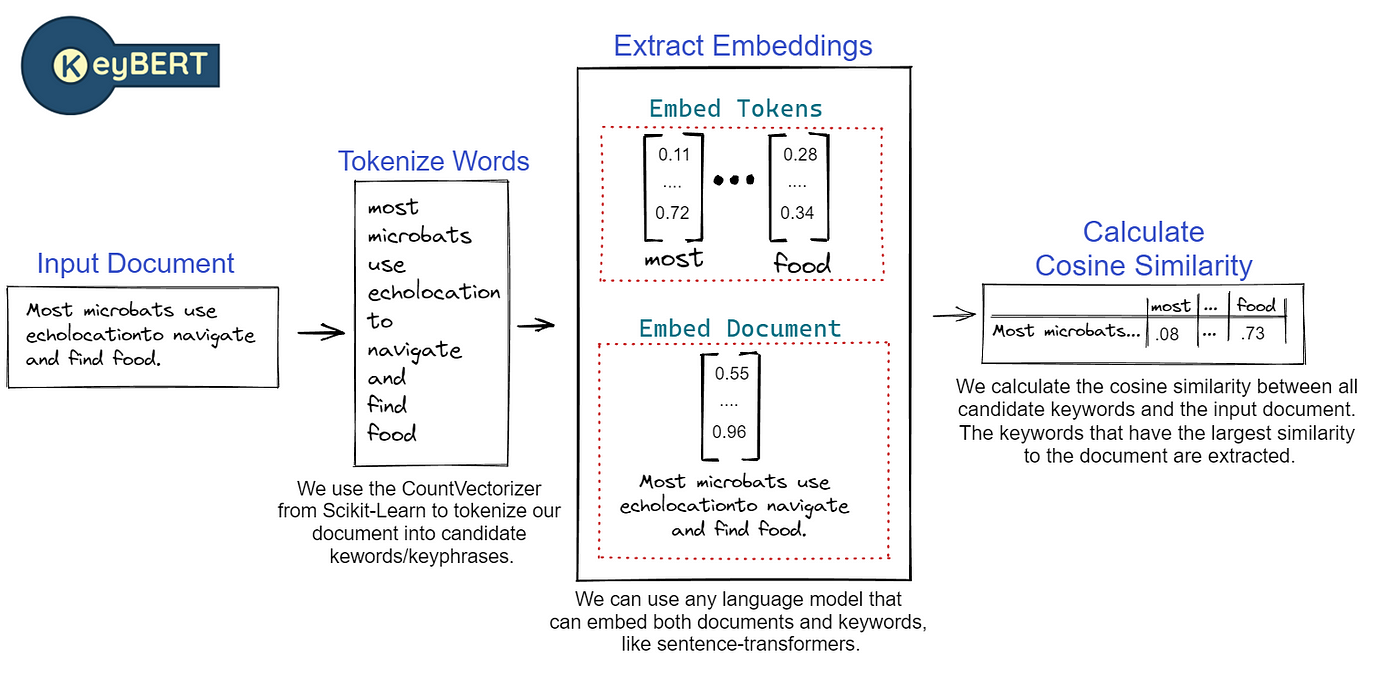
\includegraphics[width=80mm,scale=0.5]{pic/keybert.png}
    \caption{\textit{Pipeline} de la méthode \texttt{keybert} \citep{grootendorst2020keybert}.}
    \label{fig:enter-label}
\end{figure}
\end{frame}


\begin{frame}{Approches exploitant les modèles de langue -- \textit{PatternRank}}
Key\textsc{BERT} + Keyphrase-Vectorizers = \textit{\textbf{PatternRank}} \citep{schopf2022}
\begin{itemize}
\item extraction des phrases-clés les plus similaires à un document
\item préservation de leur grammaticalité grâce aux motifs POS
\end{itemize}
\begin{figure}
    \centering
    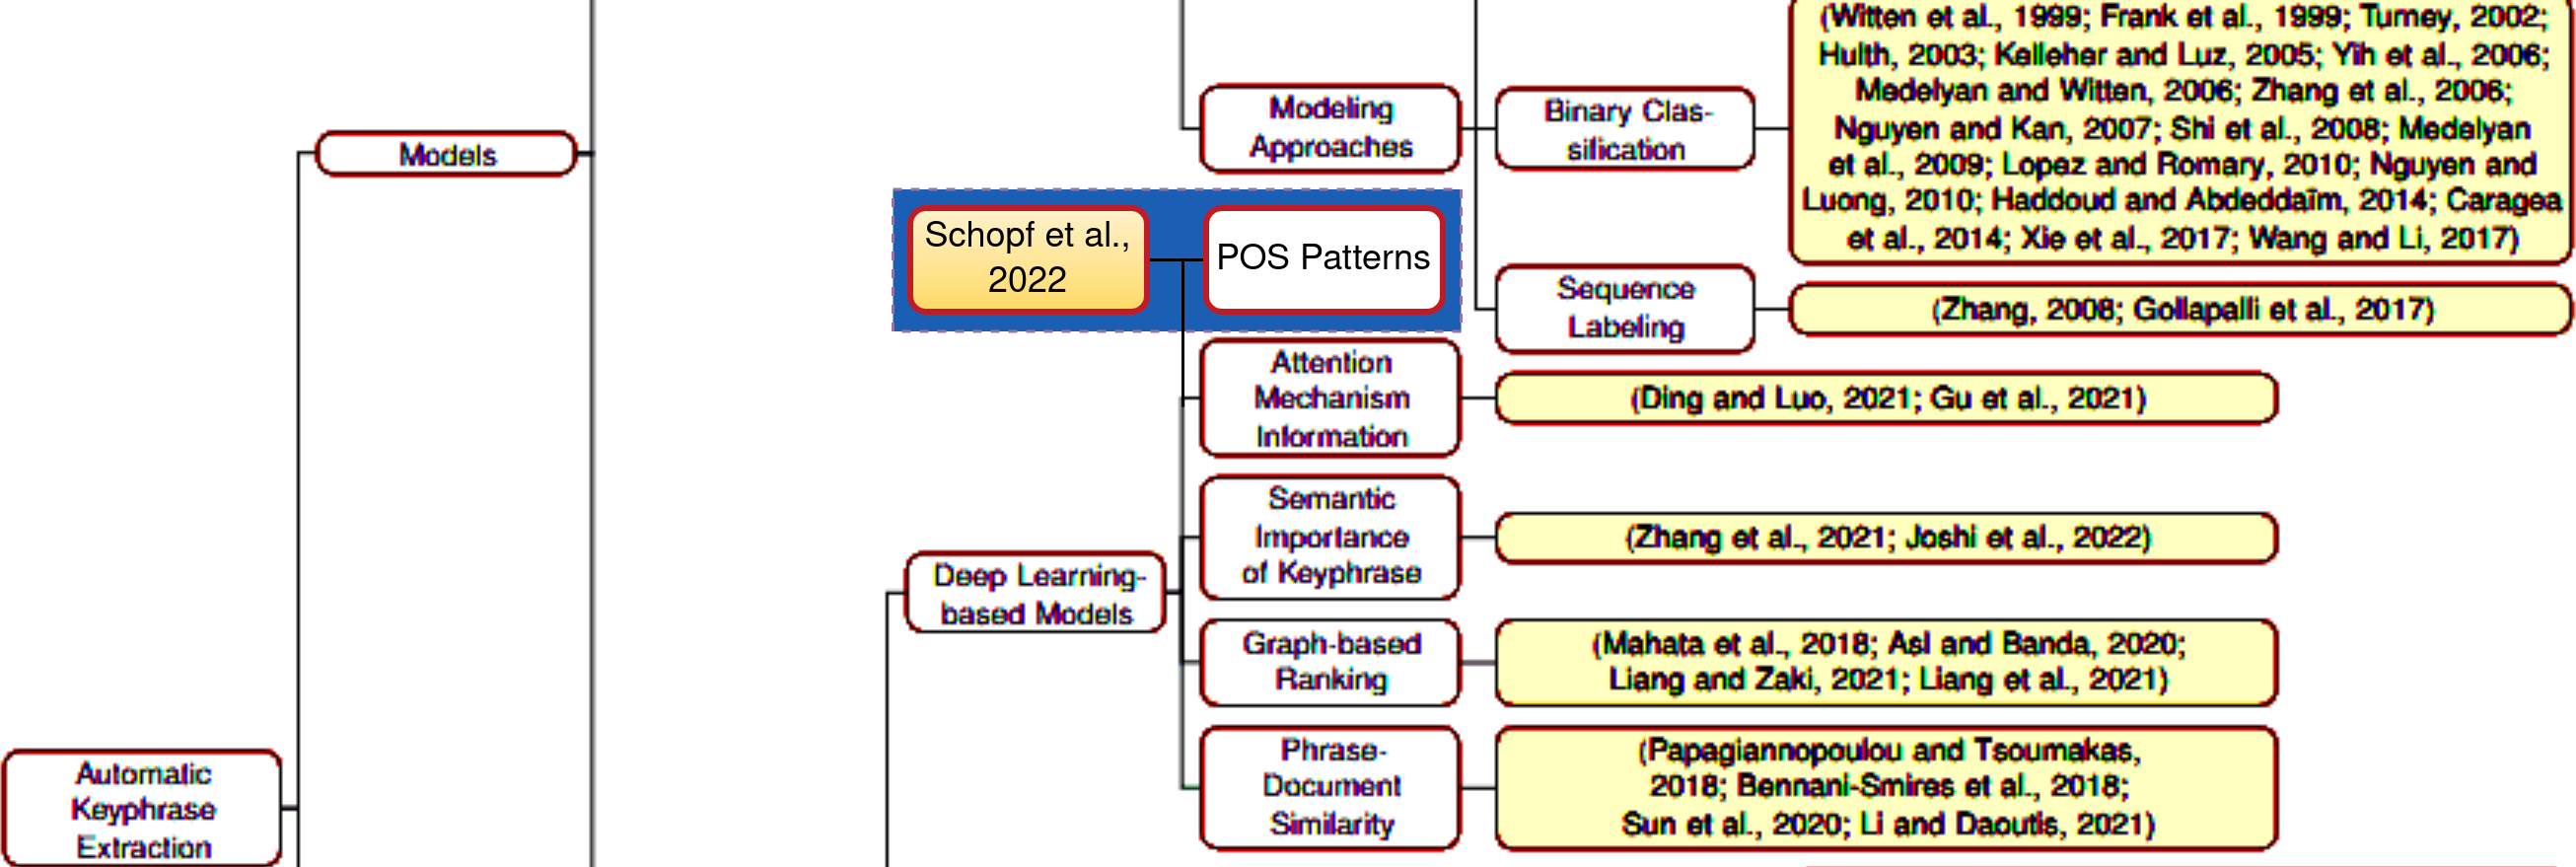
\includegraphics[width=110mm,scale=0.5]{pic/sota_lm_adapte.png}
    \caption{Extrait de l'état de l'art sur l'extraction des mots-clés, adapté de \citet{xie2023}}
    \label{fig:enter-label}
\end{figure}
\notecite{schopf2022}
\end{frame}

\begin{frame}{Fonctionnement de \textit{PatternRank}}
%\begin{itemize}
%\item extraction des phrases-clés non-supervisée
%\item exploite des modèles de langues pré-entraînés + parties du discours
%\end{itemize}
\begin{enumerate}
\item entrée : un seul document texte tokenisé
\item étiquetage des tokens avec les balises POS
\item sélection des tokens correspondant au modèle POS défini comme phrases-clés candidates
\item génération des plongements du document et des phrases-clés candidates par un modèle de langue
\item calcul des similarités cosinus entre les plongements du document et des phrases-clés candidates + classement des phrases-clés
\item extraction des \textit{N} phrases-clés les plus représentatives
\end{enumerate}
\begin{figure}
    \centering
    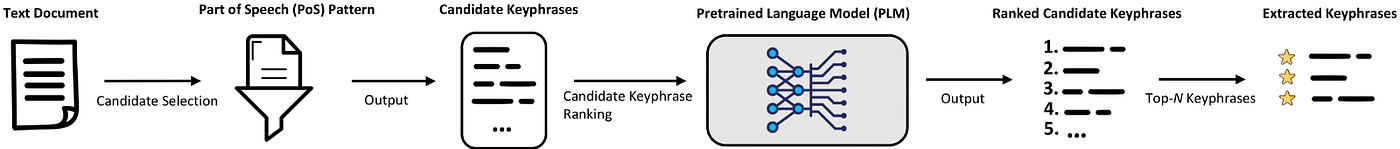
\includegraphics[width=110mm,scale=0.5]{pic/patternrank_workflow.png}
    \caption{\textit{Workflow} de la méthode \textit{PatternRank}.}
    \label{fig:enter-label}
\end{figure}
\end{frame}